\documentclass[11pt]{article}

\usepackage{fullpage}
\usepackage{mathptmx}
\usepackage[T1]{fontenc}
\usepackage{hyperref,microtype}
\usepackage{amsmath,amsfonts,amssymb,amsthm,graphicx}
\usepackage{mathtools}
\usepackage{fancyhdr}

%%% BLACKBOARD SYMBOLS

% hyperref package defines C and G, undefined to avoid conflicts
\let\C\relax
\let\G\relax
\newcommand{\C}{\ensuremath{\mathbb{C}}}
\newcommand{\D}{\ensuremath{\mathbb{D}}}
\newcommand{\F}{\ensuremath{\mathbb{F}}}
\newcommand{\G}{\ensuremath{\mathbb{G}}}
\newcommand{\J}{\ensuremath{\mathbb{J}}}
\newcommand{\N}{\ensuremath{\mathbb{N}}}
\newcommand{\Q}{\ensuremath{\mathbb{Q}}}
\newcommand{\R}{\ensuremath{\mathbb{R}}}
\newcommand{\T}{\ensuremath{\mathbb{T}}}
\newcommand{\Z}{\ensuremath{\mathbb{Z}}}
\newcommand{\QR}{\ensuremath{\mathbb{QR}}}

\newcommand{\Zt}{\ensuremath{\Z_t}}
\newcommand{\Zp}{\ensuremath{\Z_p}}
\newcommand{\Zq}{\ensuremath{\Z_q}}
\newcommand{\ZN}{\ensuremath{\Z_N}}
\newcommand{\Zps}{\ensuremath{\Z_p^*}}
\newcommand{\ZNs}{\ensuremath{\Z_N^*}}
\newcommand{\JN}{\ensuremath{\J_N}}
\newcommand{\QRN}{\ensuremath{\QR_{N}}}
\newcommand{\QRp}{\ensuremath{\QR_{p}}}

%%% THEOREM COMMANDS

\theoremstyle{plain}            % following are "theorem" style
\newtheorem{theorem}{Theorem}[section]
\newtheorem{lemma}[theorem]{Lemma}
\newtheorem{corollary}[theorem]{Corollary}
\newtheorem{proposition}[theorem]{Proposition}
\newtheorem{claim}[theorem]{Claim}
\newtheorem{fact}[theorem]{Fact}

\theoremstyle{definition}       % following are def style
\newtheorem{definition}[theorem]{Definition}
\newtheorem{conjecture}[theorem]{Conjecture}
\newtheorem{example}[theorem]{Example}
\newtheorem{protocol}[theorem]{Protocol}

\theoremstyle{remark}           % following are remark style
\newtheorem{remark}[theorem]{Remark}
\newtheorem{note}[theorem]{Note}
\newtheorem{exercise}[theorem]{Exercise}

% equation numbering style
\numberwithin{equation}{section}

%%% GENERAL COMPUTING

\newcommand{\bit}{\ensuremath{\set{0,1}}}
\newcommand{\pmone}{\ensuremath{\set{-1,1}}}

% asymptotics
\DeclareMathOperator{\poly}{poly}
\DeclareMathOperator{\polylog}{polylog}
\DeclareMathOperator{\negl}{negl}
\newcommand{\Otil}{\ensuremath{\tilde{O}}}

% probability/distribution stuff
\DeclareMathOperator*{\E}{E}
\DeclareMathOperator*{\Var}{Var}

% sets in calligraphic type
\newcommand{\calD}{\ensuremath{\mathcal{D}}}
\newcommand{\calF}{\ensuremath{\mathcal{F}}}
\newcommand{\calG}{\ensuremath{\mathcal{G}}}
\newcommand{\calH}{\ensuremath{\mathcal{H}}}
\newcommand{\calX}{\ensuremath{\mathcal{X}}}
\newcommand{\calY}{\ensuremath{\mathcal{Y}}}

% types of indistinguishability
\newcommand{\compind}{\ensuremath{\stackrel{c}{\approx}}}
\newcommand{\statind}{\ensuremath{\stackrel{s}{\approx}}}
\newcommand{\perfind}{\ensuremath{\equiv}}

% font for general-purpose algorithms
\newcommand{\algo}[1]{\ensuremath{\mathsf{#1}}}
% font for general-purpose computational problems
\newcommand{\problem}[1]{\ensuremath{\mathsf{#1}}}
% font for complexity classes
\newcommand{\class}[1]{\ensuremath{\mathsf{#1}}}

% complexity classes and languages
\renewcommand{\P}{\class{P}}
\newcommand{\BPP}{\class{BPP}}
\newcommand{\NP}{\class{NP}}
\newcommand{\coNP}{\class{coNP}}
\newcommand{\AM}{\class{AM}}
\newcommand{\coAM}{\class{coAM}}
\newcommand{\IP}{\class{IP}}

%%% "LEFT-RIGHT" PAIRS OF SYMBOLS

%% NOTE: this requires \usepackage{mathtools} in the document preamble

% inner product
\DeclarePairedDelimiter\inner{\langle}{\rangle}
% absolute value
\DeclarePairedDelimiter\abs{\lvert}{\rvert}
% a set
\DeclarePairedDelimiter\set{\{}{\}}
% parens
\DeclarePairedDelimiter\parens{(}{)}
% tuple, alias for parens
\DeclarePairedDelimiter\tuple{(}{)}
% square brackets
\DeclarePairedDelimiter\bracks{[}{]}
% rounding off
\DeclarePairedDelimiter\round{\lfloor}{\rceil}
% floor function
\DeclarePairedDelimiter\floor{\lfloor}{\rfloor}
% ceiling function
\DeclarePairedDelimiter\ceil{\lceil}{\rceil}
% length of some vector, element
\DeclarePairedDelimiter\length{\lVert}{\rVert}
% "lifting" of a residue class
\DeclarePairedDelimiter\lift{\llbracket}{\rrbracket}
\DeclarePairedDelimiter\len{\lvert}{\rvert}

%%% CRYPTO-RELATED NOTATION

% KEYS AND RELATED

\newcommand{\key}[1]{\ensuremath{#1}}

\newcommand{\pk}{\key{pk}}
\newcommand{\vk}{\key{vk}}
\newcommand{\sk}{\key{sk}}
\newcommand{\mpk}{\key{mpk}}
\newcommand{\msk}{\key{msk}}
\newcommand{\fk}{\key{fk}}
\newcommand{\id}{id}
\newcommand{\keyspace}{\ensuremath{\mathcal{K}}}
\newcommand{\msgspace}{\ensuremath{\mathcal{M}}}
\newcommand{\ctspace}{\ensuremath{\mathcal{C}}}
\newcommand{\tagspace}{\ensuremath{\mathcal{T}}}
\newcommand{\idspace}{\ensuremath{\mathcal{ID}}}

\newcommand{\concat}{\ensuremath{\|}}

% GAMES

% advantage
\newcommand{\advan}{\ensuremath{\mathbf{Adv}}}

% different attack models
\newcommand{\attack}[1]{\ensuremath{\text{#1}}}

\newcommand{\atk}{\attack{atk}} % dummy attack
\newcommand{\indcpa}{\attack{ind-cpa}}
\newcommand{\indcca}{\attack{ind-cca}}
\newcommand{\anocpa}{\attack{ano-cpa}} % anonymous
\newcommand{\anocca}{\attack{ano-cca}}
\newcommand{\euacma}{\attack{eu-acma}} % forgery: adaptive chosen-message
\newcommand{\euscma}{\attack{eu-scma}} % forgery: static chosen-message
\newcommand{\suacma}{\attack{su-acma}} % strongly unforgeable

% ADVERSARIES
\newcommand{\attacker}[1]{\ensuremath{\mathcal{#1}}}

\newcommand{\Adv}{\attacker{A}}
\newcommand{\AdvA}{\attacker{A}}
\newcommand{\AdvB}{\attacker{B}}
\newcommand{\Dist}{\attacker{D}}
\newcommand{\Sim}{\attacker{S}}
\newcommand{\Ora}{\attacker{O}}
\newcommand{\Inv}{\attacker{I}}
\newcommand{\For}{\attacker{F}}

% CRYPTO SCHEMES

\newcommand{\scheme}[1]{\ensuremath{\text{#1}}}

% pseudorandom stuff
\newcommand{\prg}{\algo{PRG}}
\newcommand{\prf}{\algo{PRF}}
\newcommand{\prp}{\algo{PRP}}

% symmetric-key cryptosystem
\newcommand{\skc}{\scheme{SKC}}
\newcommand{\skcgen}{\algo{Gen}}
\newcommand{\skcenc}{\algo{Enc}}
\newcommand{\skcdec}{\algo{Dec}}

% public-key cryptosystem
\newcommand{\pkc}{\scheme{PKC}}
\newcommand{\pkcgen}{\algo{Gen}}
\newcommand{\pkcenc}{\algo{Enc}} % can also use \kemenc and \kemdec
\newcommand{\pkcdec}{\algo{Dec}}

% digital signatures
\newcommand{\sig}{\scheme{SIG}}
\newcommand{\siggen}{\algo{Gen}}
\newcommand{\sigsign}{\algo{Sign}}
\newcommand{\sigver}{\algo{Ver}}

% message authentication code
\newcommand{\mac}{\scheme{MAC}}
\newcommand{\macgen}{\algo{Gen}}
\newcommand{\mactag}{\algo{Tag}}
\newcommand{\macver}{\algo{Ver}}

% key-encapsulation mechanism
\newcommand{\kem}{\scheme{KEM}}
\newcommand{\kemgen}{\algo{Gen}}
\newcommand{\kemenc}{\algo{Encaps}}
\newcommand{\kemdec}{\algo{Decaps}}

% identity-based encryption
\newcommand{\ibe}{\scheme{IBE}}
\newcommand{\ibesetup}{\algo{Setup}}
\newcommand{\ibeext}{\algo{Ext}}
\newcommand{\ibeenc}{\algo{Enc}}
\newcommand{\ibedec}{\algo{Dec}}

% hierarchical IBE (as key encapsulation)
\newcommand{\hibe}{\scheme{HIBE}}
\newcommand{\hibesetup}{\algo{Setup}}
\newcommand{\hibeext}{\algo{Extract}}
\newcommand{\hibeenc}{\algo{Encaps}}
\newcommand{\hibedec}{\algo{Decaps}}

% binary tree encryption (as key encapsulation)
\newcommand{\bte}{\scheme{BTE}}
\newcommand{\btesetup}{\algo{Setup}}
\newcommand{\bteext}{\algo{Extract}}
\newcommand{\bteenc}{\algo{Encaps}}
\newcommand{\btedec}{\algo{Decaps}}

% trapdoor functions
\newcommand{\tdf}{\scheme{TDF}}
\newcommand{\tdfgen}{\algo{Gen}}
\newcommand{\tdfeval}{\algo{Eval}}
\newcommand{\tdfinv}{\algo{Invert}}
\newcommand{\tdfver}{\algo{Ver}}

%%% PROTOCOLS

\newcommand{\out}{\text{out}}
\newcommand{\view}{\text{view}}

%%% COMMANDS FOR LECTURES/HOMEWORKS

\newcommand{\lecheader}{%
  \chead{\large \textbf{Lecture \lecturenum\\\lecturetopic}}

  \lhead{\small \textbf{Theory of Cryptography}\\}

  \rhead{\small \textbf{Instructor:
      \href{http://www.eecs.umich.edu/~cpeikert/}{Chris Peikert}\\Scribe:
      \scribename}}

  \setlength{\headheight}{20pt}
  \setlength{\headsep}{16pt}
}


% VARIABLES

\newcommand{\lecturenum}{9}
\newcommand{\lecturetopic}{PRPs, Symmetric Encryption}
\newcommand{\scribename}{Pushkar Tripathi}

% END OF VARIABLES

\lecheader

\pagestyle{plain}               % default: no special header

\begin{document}

\thispagestyle{fancy}           % first page should have special header

% LECTURE MATERIAL STARTS HERE

\section{Pseudorandom Permutations}
\label{sec:pseud-perm}

In the first part of this lecture we will discuss pseudorandom
\emph{permutations}.  A function $f \colon \bit^n \to \bit^n$ is said
to be a permutation if and only if it is a bijection.  Note that the
PRFs considered in the previous lecture may not be permutations.
(Exercise: construct a secure PRF family where the functions are
\emph{not} permutations.)

\subsection{Definition}
\label{sec:definition}

\begin{definition}[Pseudorandom permutation]
  \label{def:prp}
  A family of permutations $\set{f_s \colon \bit^{n} \to \bit^{n}}$ is
  a \emph{strong PRP family} (also known as ``block cipher'') if it
  is:
  \begin{itemize}
  \item \emph{Efficiently computable}: there is a deterministic
    polynomial-time algorithm $F$ such that $F(s,x) = f_s(x)$ for all
    choices of seed $s$ and input $x \in \bit^{n}$.
  \item \emph{Pseudorandom}: For every n.u.p.p.t.~$\Adv$,
    \[ \abs*{ \Pr_{f \gets \set{f_{s}} } \left[ \Adv^{f,f^{-1}}
        (1^n) = 1 \right] - \Pr_{F \gets \mathcal{P}(\bit^n)} \left[
        \mathcal A^{F,F^{-1}} (1^n) = 1 \right] } = \negl(n). \] Here
    $\mathcal{P}(\bit^n)$ is the set of \emph{all} permutations from
    $\bit^n$ to $\bit^n$, and $\Adv^{f,f^{-1}}$ denotes that the
    algorithm $\Adv$ has oracle access to both the function $f$ and
    its inverse.

    Written more succinctly using oracle indistinguishability, \[
    \left\langle f \gets \set{f_{s}} : f, f^{-1} \right\rangle
    \compind \left\langle F \gets \mathcal{P}(\bit^{n}) : F, F^{-1}
    \right\rangle. \]
  \end{itemize}
  
  We say that the family is a \emph{weak} PRP family if it is
  pseudorandom in the forward direction, i.e., if the pseudorandomness
  condition holds when the adversary is given oracle access to only
  $f$ (or $F$), and not their inverses.
\end{definition}

\subsection{Feistel Construction}
\label{sec:feistel-construction}

Perhaps surprisingly, a PRP family can be obtained from any PRF family
(even though the functions in the PRF family may not themselves be
permutations!).  To accomplish this, we first show a way to obtain a
permutation from \emph{any} (length-preserving) function $f$; this
process is called a \emph{Feistel round}, after its inventor.  (One
can think of $f$ as being drawn from a PRF family, though the Feistel
construction makes no complexity assumption on $f$.)

\begin{definition}
  \label{def:feistel-round}
  For a function $f \colon \bit^{n} \to \bit^{n}$, the Feistel
  function $\mathcal D_f : \bit^{2n} \rightarrow \bit^{2n}$ is defined
  as follows:
  \[ D_f(L, R) = (R,L \oplus f(R) ). \]
\end{definition}

Figure~\ref{fig:feistel_1_pic} gives a pictorial representation of
this construction.

\begin{center}
  \centering
  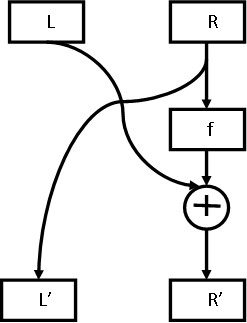
\includegraphics[width=0.20\textwidth]{feistel1.png}
  \label{fig:feistel_1_pic}
\end{center}

Note that for $L'$ and $R'$ as defined above, we have $L = f(L')
\oplus R'$ and $R = L'$.  Thus the function $D_f$ is invertible, and
hence defines a bijection.  Formally, we can write $D_{f}^{-1} = \rho
\circ D_f \circ \rho$, where $\rho(L,R) = (R,L)$.

However, $D_{f}$ by itself does \emph{not} define a PRF.  This is
because $\textsc{LEFT}( D_f(L,R) ) = R$ for any $L,R$, which is rarely
be the case for a truly random permutation.  But what happens if we
use \emph{two} Fesitel rounds, each with a (possibly different) round
function (see Figure~\ref{fig:feistel_2_pic})?

\begin{center}
  \centering
  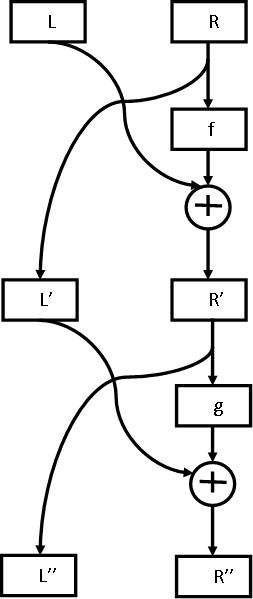
\includegraphics[width=0.20\textwidth]{feistel2.png}
  \label{fig:feistel_2_pic}
\end{center}

Unfortunately, two Feistel rounds also does not yield a PRP family.
Consider arbitrary $L_1, L_2, R \in \bit^n$ with $L_{1} \neq L_{2}$,
and any function $f : \bit^n \rightarrow \bit^n$.  We have
$\textsc{Right}( D_f(L_1,R) ) = L_1\oplus f(R) $ and
$\textsc{Right}(D_f(L_2,R) ) = L_2\oplus f(R)$.  Taking the
exclusive-or of both equations, we get \[ \textsc{Right}( D_f(L_1,R))
\oplus \textsc{Right}( D_f(L_2,R)) = L_1 \oplus L_2. \] On the other
hand, for a truly random permutation $\mathcal P$, $\mathcal P(L_1,R)
\oplus \mathcal P(L_2, R)$ is the exclusive-or of two distinct random
strings and its right half would equal $L_1\oplus L_2$ with only
negligible probability.

Fortunately, all is not lost: we have the following theorem of Luby
and Rackoff.

\begin{theorem}[Luby-Rackoff Theorem]
  \label{thm:luby-rackoff}
  Three rounds of the Feistel construction, each with a round function
  drawn independently from a  PRF family, yields a \emph{weak} PRP
  family.  Moreover, four rounds yields a \emph{strong} PRP family.
\end{theorem}

\subsection{Historical Notes}
\label{sec:historical-notes}

The Data Encryption Standard (DES) from 1977 is a Feistel
construction, but with dependent and only ``weakly'' pseudorandom
round functions.  The Feistel idea predates any rigorous definitions
or analysis.  A large fraction of fast block ciphers use a Feistel
network, though more recently designers have started using other
structures.  For example, the Advanced Encryption Standard (AES) is
not based on a Feistel network.

\section{Security for Shared-Key Encryption}
\label{sec:security-shared-key}

We now take the first steps towards building a secure shared-key
(symmetric) encryption system.  Before we proceed, recall the model
for a shared-key cryptosystem, which is represented by a triple of
algorithms $(\skcgen, \skcenc,\skcdec)$, where
\begin{itemize}
\item $\skcgen$ is a randomized algorithm that takes no input (aside
  from the implicit security parameter $1^{n}$), and outputs a key $k$
  in some (finite) set $\keyspace$.
\item $\skcenc_k(m) = \skcenc(k,m)$ takes a key $k \in \keyspace$ and
  message $m \in \msgspace$, and outputs a ciphertext $c \in
  \ctspace$.
\item $\skcdec_k(c) = \skcdec(k, c)$ takes a key $k \in \keyspace$ and
  ciphertext $c \in \ctspace$, and outputs a message $m \in
  \msgspace$.
\end{itemize}

Also recall the definition of perfect secrecy.

\begin{definition}
  A shared-key encryption scheme $(\skcgen, \skcenc, \skcdec)$ with
  message space $\msgspace$ and ciphertext space $\ctspace$ is
  \textit{perfectly secret} if for all $m_0, m_1 \in \msgspace$ and
  all $\bar{c} \in \ctspace$,
  \[ \Pr_{k \gets Gen} \left[ \skcenc_k(m_0) = \bar{c} \right] =
  \Pr_{k \gets Gen} \left[ \skcenc_k(m_1) = \bar{c} \right]. \] That
  is, the distributions of $\skcenc_{k}(m_{0})$ and
  $\skcenc_{k}(m_{1})$ are \emph{identical}, over the choice of the
  key $k \gets \skcgen$.
\end{definition}

\subsection{A Computational Analogue of Perfect Secrecy}
\label{sec:comp-anal-perf}

The definition of perfect secrecy suggests a natural analogue for the
computational setting.

\begin{definition}[Single-message indistinguishability]
  \label{def:single-msg-indist}
  An encryption scheme satisfies \emph{single-message
    indistinguishability} if for all messages $m_0,m_1 \in \msgspace$,
  \[ \left\{ k \gets \skcgen : \skcenc_k(m_0) \right\} \compind
  \left\{ k \gets \skcgen : \skcenc_k(m_1) \right\}. \]
\end{definition}

The following lemma follows immediately. 

\begin{lemma}
  \label{lem:pseudorand-one_msg_secure}
  For a symmetric encryption scheme $\skc$, if $\set{k \gets \skcgen :
    \skcenc_k(m)}$ is pseudorandom over $\ctspace$ for every $m \in
  \msgspace$, then the scheme is single-message indistinguishable.
\end{lemma}

\begin{proof}
  Fix any two messages $m_0, m_1 \in \msgspace$.  Using the definition
  of pseudorandomness, we have
  \[ \left\{ \skcenc_k(m_0) \right\} \compind \left\{ U(\ctspace)
  \right\} \compind \left\{ \skcenc_k(m_1) \right\}. \] By the
  \emph{hybrid lemma} we have $ \left\{ \skcenc_k(m_0) \right\}
  \compind \left\{ \skcenc_k(m_1) \right\}$, as desired.
\end{proof}

Now we describe a symmetric encryption scheme, and use
Lemma~\ref{lem:pseudorand-one_msg_secure} to prove its one-message
security.  Let $\keyspace = \bit^n$ be the keyspace, and let
$\msgspace = \bit^{\ell(n)}$ be the message space, where $\ell(n)$ is
a polynomial in $n$.  Let $G$ be a PRG with output length $\ell(n)$.
The following algorithms specify the encryption scheme.
\begin{itemize}
\item $\skcgen$ outputs a uniformly random $k \gets \bit^{n}$.
\item $\skcenc_k(m) = \skcenc(k,m)$ outputs $c = m \oplus G(k)$.
\item $\skcdec_k(c) = \skcdec(k, c)$ outputs $m = c \oplus G(k)$.
\end{itemize}

\begin{claim}
  For any $m \in \bit^{\ell(n)}$, the distribution of ciphertexts
  $\left\{ k \gets \skcgen : \skcenc_k(m) \right\}$ produced by the
  above scheme is pseudorandom.
\end{claim}

\begin{proof}
  \begin{eqnarray}
    \left\{ k \gets \skcgen : \skcenc_k(m) \right\} & \equiv &
    \left\{ k \gets \bit^{n} : m \oplus G(k) \right\} \label{eq:scheme} \\
    & \compind & \left\{ x \gets U_{\ell(n)} : m \oplus x
    \right\} \label{eq:prg} \\
    & \equiv & \left\{ U_{\ell(n)} \right\}. \label{eq:prob}
  \end{eqnarray}
  Equation~\eqref{eq:scheme} is by definition of the scheme.
  Equation~\eqref{eq:prg} is true because $G$ is a PRG, and by a
  trivial simulation.  Equation~\eqref{eq:prob} is by basic
  probability.
\end{proof}

Note that the scheme constructed above is good for encrypting only
\emph{one} message; it would fail completely if we encrypt two
different messages using the same key.  For example, consider $m_0,
m_1 \in \msgspace$ that are encrypted using the above scheme with the
same key $k \in \keyspace$.  Then we have $\skcenc_k(m_0) = m_0 \oplus
G(k)$ and $\skcenc_k(m_1) = m_1 \oplus G(k)$.  Taking the exclusive-or
of these two ciphertexts, we get $m_0 \oplus m_1$.  In many cases
(such as when the two messages are English prose), this is enough
information to recover the two messages completely!

A possible way to counter the problem is to encrypt every message with
a different key.  But this would require the two communicating parties
to have a large set of predecided secret keys.  Alternatively, we
might modify the encryption algorithm to append to its message a fresh
key that would be used to encrypt the subsequent message (note that
this is possible because the message length is longer than the key
length, which is something we could not achieve with perfect secrecy).
But this method also suffers from a drawback: the encryption and
decryption algorithms are \emph{stateful}.  If even a single message
fails to reach the receiver, it might cause the entire scheme to
become out of sync.

More fundamentally, though, before thinking about ways to securely
encrypt multiple messages, we first need a \emph{definition} of
security that captures this intended mode of usage.

\subsection{Multiple-Message Indistinguishability}
\label{sec:mult-mess-indist}

\begin{definition}[Multi-message indistinguishability]
  \label{def:multi-msg-indist}
  An encryption scheme is multi-message indistinguishable if for all
  $q=\poly(n)$ and all message tuples $\left( m_0, m_1 \cdots m_q
  \right) \in \msgspace^q$ and $\left( m'_0, m'_1 \cdots m'_q \right)
  \in \msgspace^q$, we have
  \[ \left( \skcenc_k(m_0), \skcenc_k(m_1) \cdots \skcenc_k(m_q)
  \right) \compind \left( \skcenc_k(m'_0), \skcenc_k(m'_1) \cdots
    \skcenc_k(m'_q) \right), \] where both experiments are over $k
  \gets \skcgen$ and any randomness of $\skcenc$.
\end{definition}

\begin{remark}
  For multi-message indistinguishability, $\skcenc$ cannot be
  \emph{deterministic}.  Otherwise, it would be trivial to distinguish
  between the encryptions of a tuple with identical messages and one
  without, since $\skcenc_{k}(m)$ would always produce the same
  ciphertext given the same message.  Therefore, $\skcenc$ must either
  be \emph{randomized} or \emph{stateful}.
\end{remark}

Unfortunately, we are still not done.  In order to make our definition
completely water-tight, we need to capture some additional (realistic)
power of the adversary: that it may be able to influence the choice of
messages that are encrypted.  Specifically, the adversary may have the
power to \textbf{adaptively} choose these encrypted messages, based on
its view of the prior ciphertexts. 

\subsection{Indistinguishability under (Adaptive) Chosen-Plaintext Attack}
\label{sec:indist-under-chos}

The above considerations prompt us to adopt
\textit{indistinguishability under (adaptive) chosen-plaintext attack
  (IND-CPA)} as our notion of security.  Before giving a precise
definition of security, we list some of the aspects that the
definition should capture.

\begin{itemize}
\item We allow the adversary $\Adv$ to \emph{adaptively} query the
  encryption oracle, based on the ciphertexts it has already seen.
\item We still want indistinguishability between the encryptions of
  two messages (also chosen by $\Adv$).
\end{itemize}

Now we present a formal definition satisfying the above goals.

\begin{definition}[IND-CPA security]
  \label{def:ind-cpa}
  An encryption scheme is said to be IND-CPA secure if the following
  pairs of oracles are computationally indistinguishable:
  \[ \left\langle k \gets \skcgen : C^0_k(\cdot, \cdot) \right\rangle
  \compind \left\langle k \gets \skcgen : C^1_k(\cdot, \cdot)
  \right\rangle. \] Here $C^{b}_{k}(m_{0}, m_{1})$, called the
  \emph{challenge oracle}, simply runs $\skcenc_{k}(m_{b})$ and
  outputs the result, using fresh randomness (or keeping any state)
  with each invocation.
\end{definition}

Observe that the only difference between the two oracles is in the bit
$b$ used by the challenger, i.e., which message is encrypted to
produce the challenge ciphertext.  Also observe that given access to
either $C^{b}_{k}(\cdot,\cdot)$, we have implicit access to
$\skcenc_{k}(\cdot)$ just by querying $C^{b}_{k}$ on two equal
messages.

\begin{exercise}
  Show that IND-CPA security implies
  multi-message security, but the converse is false.  \textit{Hint:}
  Define a ``pathological'' scheme that gives away its secret key via a
  certain sequence of adaptive queries.
\end{exercise}

We now describe a PRF-based encryption scheme enjoying IND-CPA
security.  Define $\keyspace = \msgspace = \bit^{n}$ for the
encryption scheme, and assume that $\set{f_{k} \colon \bit^{n} \to
  \bit^{n}}_{k \in \bit^{n}}$ is a PRF family.
\begin{itemize}
\item $\skcgen$: output $k \gets \bit^n$.
\item $\skcenc_k(m)$: choose $r \gets U_n$ and output $(r, f_k(r)
  \oplus m)$ as the cipher text.
\item $\skcdec_k(r,c)$: output $f_k(r) \oplus c$ as the decrypted
  message.
\end{itemize}

It is easy to observe that the scheme is correct,
i.e. $\skcdec_k(\skcenc_k (m)) = f_k(r) \oplus f_k(r) \oplus m =
m$. In the next lecture we will prove that this scheme is IND-CPA
secure.

\end{document}

%%% Local Variables: 
%%% mode: latex
%%% TeX-master: t
%%% End: 
